% !TEX root = ../main.tex
\begin{figure*}[t]
  \centering
  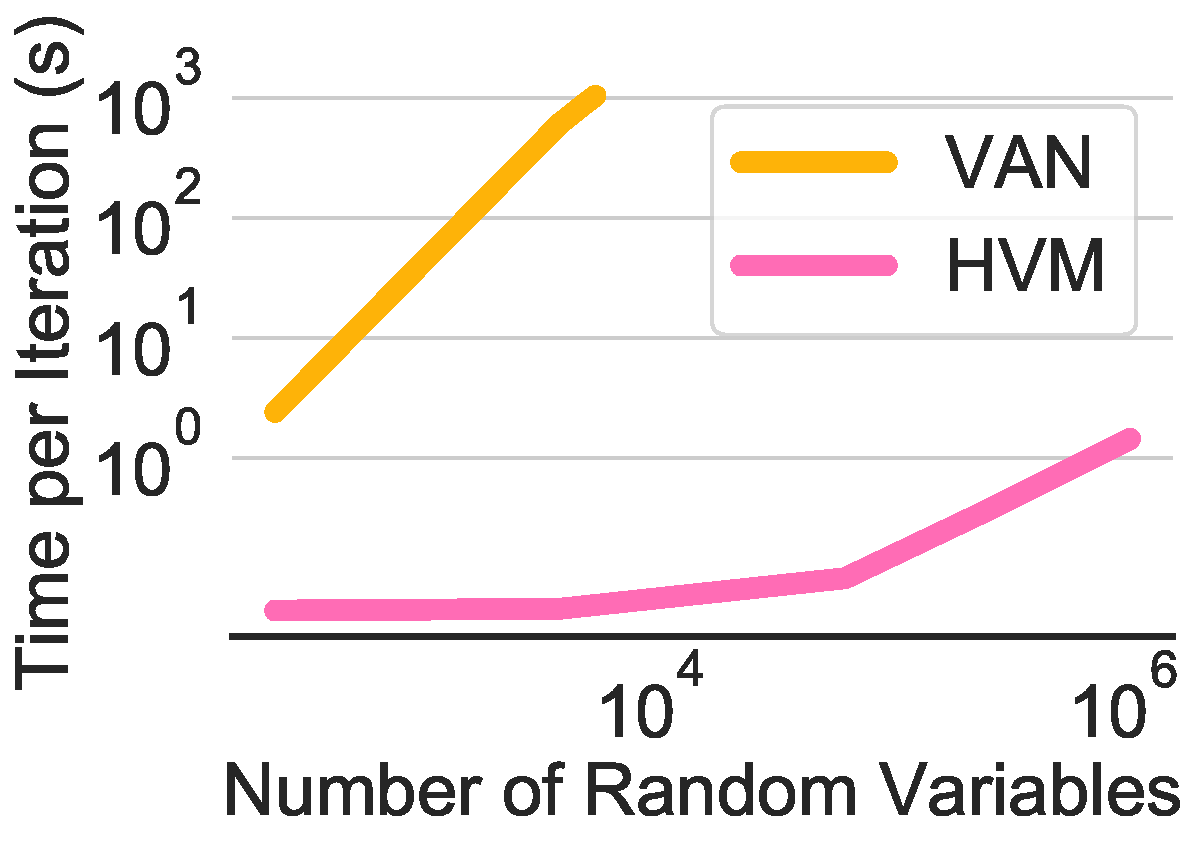
\includegraphics[width=0.5\textwidth]{fig/ising-scaling.pdf}
  \caption[Comparing scaling of \textsc{hvm}s to \textsc{van}s in large systems]{\textbf{\Acrfullpl{hvm} are faster than \Acrfullpl{van} \citep{wu2019solving} and scale to larger systems.} The scaling of both variational approximations is illustrated with the time taken per iteration in Ising models. The \gls{hvm} variational approximations use $5400$ parameters and the \gls{van} method uses over $700$k. The \gls{van} approximation runs out of memory with $16384$ random variables, while the \gls{hvm} method scales to models with over $1$M random variables.}
  \label{fig:ising-scaling}
\end{figure*}